\subsection{UC4 – Gestione Risultati}
\begin{center}
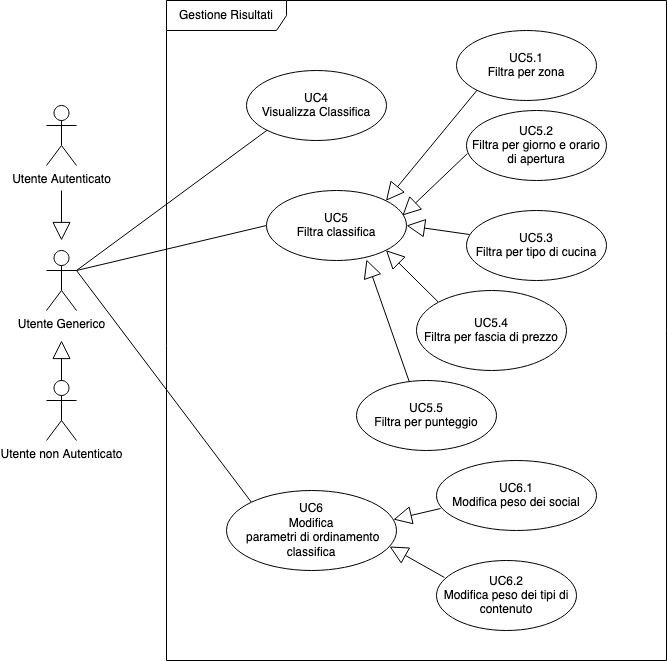
\includegraphics[scale=0.5]{UC_images/UC4.png}
\end{center}
\subsubsection{UC4.1 – Visualizza Classifica}
\begin{center}
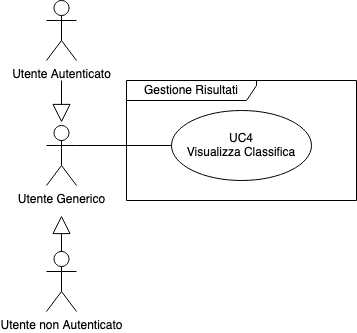
\includegraphics[scale=0.5]{UC_images/UC4-2.png}
\end{center}
\begin{itemize}
    \item \textbf{Attore primario}: Utente autenticato.
    \item \textbf{Precondizione}: L’utente si trova all’interno della piattaforma Sweeat.
    \item \textbf{Postcondizione}: L’utente visualizza a schermo la classifica dei migliori locali gastronomici prodotta dal sistema senza alcun filtro applicato e con i parametri di ordinamento di default.
    \item \textbf{Scenario principale}: 
    \begin{enumerate}
        \item Un utente generico accede al sistema;
        \item L’utente seleziona la funzionalità visualizza classifica.
    \end{enumerate}
\end{itemize}

